\documentclass[xcolor=pdftex,dvipsnames,table]{beamer}
\usepackage{tikz}
\usetikzlibrary{arrows, shapes.geometric, decorations.markings}

\begin{document}
\begin{frame}
\frametitle{Loss Latency Tradeoff}

  \begin{columns}
    \begin{column}{0.6\textwidth}

\begin{center}

\begin{table}
  \rowcolors{1}{RoyalBlue!20}{RoyalBlue!5}
  \begin{tabular}{l | c | c | c | c }
    run & mean & min & max & stddev \\
    \hline \hline
    CTL & 15.48 & 5 & 24 & 5.18609\\ 
    EXP & 4.32 & 4 & 6 & 0.509243\\
  \end{tabular}
  \caption{real-time flow latency (ms)}
\end{table}

\begin{table}
  \rowcolors{1}{RoyalBlue!20}{RoyalBlue!5}
  \begin{tabular}{l | c | c | c | c }
    run & honest & liar \\
    \hline \hline
    CTL & 2.01904 & 1.837216\\ 
    EXP & 2.399816 & 1.332176\\
  \end{tabular}
  \caption{TCP flow throughput (Mbps)}
\end{table}

\end{center}

\end{column}


\begin{column}{0.5\textwidth}
  \begin{center}
    \resizebox{6cm}{6cm}{
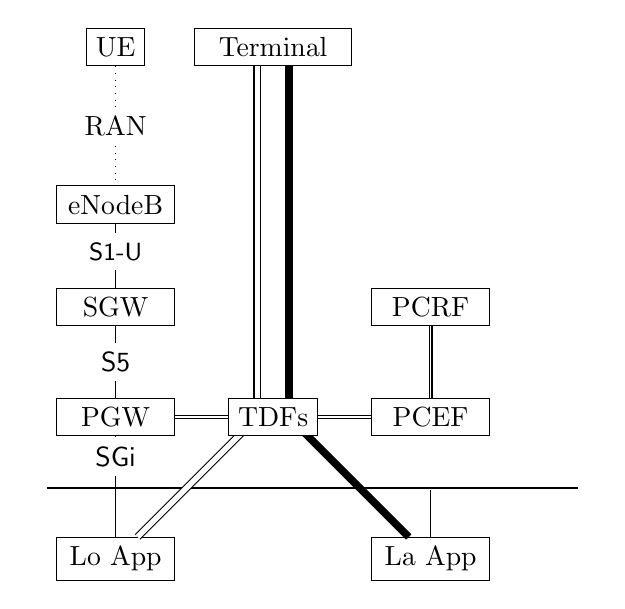
\begin{tikzpicture}[auto, node distance=2cm,>=latex']
  \node (ue) at (0,0) [draw,rectangle] {UE};
  \node (l) at (2,0) {}; % invisible node
  \node (l1) at (1.8,0) {}; % invisible node
  \node (l2) at (2.2,0) {}; % invisible node
  \node (eb) at (0,-2) [draw,rectangle, minimum width=1.5cm]{eNodeB};
  \node (sgw) at (0,-3.3) [draw,rectangle, minimum width=1.5cm] {SGW};
  \node (pgw) at (0,-4.7) [draw,rectangle, minimum width=1.5cm] {PGW};
  \node (k) at (2,-4.7) {}; % invisible node
  \node (k1) at (1.8,-4.7) {}; % invisible node
  \node (k2) at (2.2,-4.7) {}; % invisible node
  \node (pcef) at (4,-4.7) [draw,rectangle, minimum width=1.5cm] {PCEF};
  \node (pcrf) at (4,-3.3) [draw,rectangle, minimum width=1.5cm] {PCRF};

  %% SGi LAN
  \node (a) at (-1,-5.6) {}; % invisible node
  \node (b) at (6,-5.6) {}; % invisible node
  \node (c) at (0,-5.6) {}; % invisible node
  \draw[black] (a) -- (b);

  \node (app) at (0,-6.5) [draw,rectangle, minimum width=1.5cm]{Lo App};
  \node (d)   at (0,-5.5) {}; % invisible node
  \node (laa) at (4,-6.5) [draw,rectangle, minimum width=1.5cm]{La App};
  \node (e)   at (4,-5.5) {}; % invisible node


  \draw[black] (eb) to (sgw);
  \draw[black] (sgw) to (pgw);
  \draw[black] (pgw) to (app);
  \draw[black] (e) to (laa);

  \draw[double] (pgw) to (pcef);
  \draw[double] (pcrf) to (pcef);
  \draw[dotted] (ue) to (eb);% {RAN} (ran);

  \draw [black,thin,double distance=2pt,double=white] (l1) to (k1);
  \draw [black,thin,double distance=2pt,double=black] (l2) to (k2);
  \draw [black,thin,double distance=2pt,double=white] (k1) to (app);
  \draw [black,thin,double distance=2pt,double=black] (k2) to (laa);

  \node (tdfs) at (2,-4.7) [draw,rectangle,fill=white] {TDFs};
  \node (apps) at (2,0) [draw,rectangle,fill=white, minimum width=2cm] {Terminal};
  \node (sgi) at (0,-1) [draw=white,fill=white]{RAN};
  \node (sgi) at (0,-5.2) [draw=white,fill=white]{\textsf{SGi}};
  \node (s1u) at (0,-2.6) [draw=white,fill=white]{\textsf{\small{S1-U}}};
  \node (s5) at (0,-4) [draw=white,fill=white]{\textsf{S5}};
\end{tikzpicture}
}

  \end{center}
\end{column}
\end{columns}
\end{frame}
\end{document}
